\documentclass{article}
\usepackage[T1,T2A]{fontenc}
\usepackage[utf8]{inputenc}
\usepackage[english,russian]{babel}
\usepackage{amsmath}
\usepackage{amsfonts}
\usepackage{amssymb}
\usepackage{makeidx}
\usepackage{listings}
\usepackage{setspace,amsmath}
\usepackage{graphicx}%Вставка картинок правильная
\usepackage{float}%"Плавающие" картинки
\usepackage{wrapfig}

\begin{document}

\begin{titlepage}
	\newpage
	
	\begin{center}
		\textbf{Федеральное государственное бюджетное образовательное учреждение высшего образования «Московский государственный университет имени М. В. Ломоносова»}\\
	\end{center}
	
	\vspace{8em}
	
	\begin{center}
		\Large Кафедра вычислительной механики \\ 
	\end{center}
	
	\vspace{2em}
	
	\begin{center}
		\Large \textsc{\textbf{Отчёт по задаче на работу с изображениями по теме:}}
		\\
		\Large \textsc{\textbf{ Фрактальное сжатие изображений \linebreak}}
	\end{center}
	
	\vspace{15em}
	
	
	
	\begin{flushright}
		\small
		\textbf{Преподаватель: Почеревин Роман Владимирович}\\
		\textbf{Студент 223 группы: Скворцов Андрей Сергеевич}\\
	\end{flushright}
	
	
	\vspace{\fill}
	
	\begin{center}
		Москва \\2024
	\end{center}
	
\end{titlepage}

\begin{center}

{\large\bf Отчёт по работе с BMP-изображениями в Python-3}

\end{center}

\textit{З\,а\,д\,а\,н\,и\,е.} Реализовать алгоритмы фрактального сжатия и восстановления изображения.

 
\textit{Р\,е\,ш\,е\,н\,и\,е.}  Используя библиотеки numpy и scipy, можно решить эту задачу проще. Кроме того используем библиотеки multiprocessing для распараллеливания программы:

\section{Загрузка изображений}

{\usefont{T2A}{cmss}{m}{n}
\hspace{1cm}	import matplotlib.pyplot as plt
	
\hspace{1cm}	import matplotlib.image as mpimg
	
\hspace{1cm}	from scipy import ndimage
	
\hspace{1cm}	import numpy as np
	
\hspace{1cm}	from PIL import Image
	
\hspace{1cm}	import multiprocessing as mp
	
\hspace{1cm}	import datetime 

}
\vspace{1em}

Пусть изображения заданы внутри программы. Выгрузим его как черно-белое при помощи функции get\_greyscale\_image(img):
{\usefont{T2A}{cmss}{m}{n}

def get\_greyscale\_image(img):

\hspace{1cm}		return np.mean(img[:,:,:2], 2)
}
Далее разобьем изображение на нужные нам блоки размера 4 на 4 вместо 8 на 8 при помощи функции reduce(img, factor):
{\usefont{T2A}{cmss}{m}{n}

def reduce(img, factor):

\hspace{1cm}	result = np.zeros((img.shape[0] // factor, img.shape[1] // factor))

\hspace{1cm}	for i in range(result.shape[0]):

\hspace{2cm}		for j in range(result.shape[1]):

\hspace{3cm}			result[i, j] = np.mean(img[i * factor:(i + 1) * factor,j * factor:(j + 1) * factor])


\hspace{1cm}	return result
}
\vspace{1em}

\section{Алгоритм фрактального сжатия}

\subsection{Генерация преобразованных блоков}

Теперь рассмотрим сам алгоритм фрактального сжатия изображения. Оно происходит при вызове функции compress. Сначала мы генерируем всевозможные блоки, которые мы можем получить при помощи нашего отображения, при помощи
функции generate\_all\_transformed\_blocks:
 
{\usefont{T2A}{cmss}{m}{n}
def generate\_all\_transformed\_blocks(img, source\_size\_block, destination\_size\_block, step):

\hspace{1cm}		factor = source\_size\_block // destination\_size\_block

\hspace{1cm}		transformed\_blocks = []

\hspace{1cm}		for k in range((img.shape[0] - source\_size\_block) // step + 1):

\hspace{2cm}			for l in range((img.shape[1] - source\_size\_block) // step + 1):

\hspace{3cm}				\# Преобразуем исходный блок в конечный (доменный -> ранговый)

\hspace{3cm}				S = reduce(img[k * step:k * step + source\_size\_block,l * step:l * step + source\_size\_block], factor)

\hspace{3cm}				\# Всевозможные преобразования при помощи найшего сжимающего изображения

\hspace{3cm}				for direction, angle in candidates:

\hspace{4cm}					transformed\_blocks.append((k, l, direction, angle, apply\_transformation(S, direction, angle)))

\hspace{1cm}		return transformed\_blocks
}
\vspace{1em}

В этой функции мы исползуем функции поворота на угол кратный пи / 2 и отзеркаливание блока с последующим примением трансформации:

{\usefont{T2A}{cmss}{m}{n}
def rotate(img, angle):

\hspace{1cm}	return ndimage.rotate(img, angle, reshape = False)

def flip(img, direction): \# Отражает изображение зеркально, если direction равно -1 и не отражает, если значение равно 1
\hspace{1cm}	return img[::direction,:]

def apply\_transformation(img, direction, angle, contrast = 1.0, brightness = 0.0): \# сжимающее отображение

\hspace{1cm}	return contrast * rotate(flip(img, direction), angle) + brightness
}
\vspace{1em}

\subsection{Алгоритм фрактального сжатия}

Далее для каждого блока размером 8 на 8 ищем наиболее похожий на него блок размера 4 на 4 и сохраняем параметры преобразования этого блока, а также координаты исходного блока:

{\usefont{T2A}{cmss}{m}{n}
def compress(img, source\_size\_block, destination\_size\_block, step):

\hspace{1cm}		transformations = []

\hspace{1cm}		transformed\_blocks = generate\_all\_transformed\_blocks(img, source\_size\_block, destination\_size\_block, step) \# Генерируем всевозможные преобразования

\hspace{1cm}		i\_count = img.shape[0] // destination\_size\_block

\hspace{1cm}		j\_count = img.shape[1] // destination\_size\_block

\hspace{1cm}		for i in range(i\_count):

\hspace{2cm}			transformations.append([])

\hspace{2cm}			for j in range(j\_count):

\hspace{3cm}				transformations[i].append(None)

\hspace{3cm}				min\_d = float('inf')

\hspace{3cm}				\# Берем доменный блок

\hspace{3cm}				D = img[i * destination\_size\_block:(i + 1) * destination\_size\_block,j * destination\_size\_block:(j + 1) * destination\_size\_block]

\hspace{3cm}				\# Выбираем самый похожий блок

\hspace{3cm}				for k, l, direction, angle, S in transformed\_blocks:

\hspace{4cm}					contrast, brightness = find\_contrast\_and\_brightness2(D, S)

\hspace{1cm}					S = contrast * S + brightness

\hspace{4cm}				d = np.sum(np.square(D - S)) \# Сумма квадратов D - S (типа square это поэлементый квадрат)

\hspace{4cm}				\# Ищем самый похожий блок

\hspace{4cm}				if d < min\_d:

\hspace{5cm}					min\_d = d

\hspace{5cm}					transformations[i][j] = (k, l, direction, angle, contrast, brightness)

\hspace{5cm}					transformations\_no\_fratal[i][j] = S

\hspace{1cm}	np.save('save\_data\_{}'.format(number), transformations\_no\_fratal)

\hspace{1cm}	np.save('save\_data\_fractal\_{}'.format(number), transformations)

\hspace{1cm}	return transformations
}
\vspace{1em}

Для наибольшей схожести блоков подбираем яркость и контрастность при помощи функции find\_contrast\_and\_brightness2, причем схожесть определяется методом наименьших квадратов, реализованным в библиотеке numpy:
{\usefont{T2A}{cmss}{m}{n}
def find\_contrast\_and\_brightness2(D, S):

\hspace{1cm}	A = np.concatenate((np.ones((S.size, 1)), np.reshape(S, (S.size, 1))), axis = 1) \# Объединение массивов вдоль оси

\hspace{1cm}	b = np.reshape(D, (D.size,))

\hspace{1cm}	x, \_, \_, \_ = np.linalg.lstsq(A, b, rcond=None) \# Решение матричного уравнения методом наименьших квадратов

\hspace{1cm}	return x[1], x[0]
}

\vspace{1em}

\subsection{Восстановление изображения после фрактального сжатия}

Теперь рассмотрим алгоритм восстановления описанный в функции decompress. Самое полезное для нас в сжимающем отображении это наличие неподвижных точек в каждом блоке, поэтому для восстановления изображения 
нужно просто применить это отображение несколько раз к случайному изображению:

{\usefont{T2A}{cmss}{m}{n}
def decompress(transformations, source\_size\_block, destination\_size\_block, step, nb\_iter = 8):

\hspace{1cm}	factor = source\_size\_block // destination\_size\_block

\hspace{1cm}	height = len(transformations) * destination\_size\_block

\hspace{1cm}	width = len(transformations[0]) * destination\_size\_block

\hspace{1cm}	iterations = [np.random.randint(0, 256, (height, width))]

\hspace{1cm}	cur\_img = np.zeros((height, width))

\hspace{1cm}	for i\_iter in range(nb\_iter):

\hspace{2cm}		for i in range(len(transformations)):

\hspace{3cm}			for j in range(len(transformations[i])):

\hspace{4cm}				\# Применяем отображение

\hspace{4cm}				k, l, flip, angle, contrast, brightness = transformations[i][j]

\hspace{4cm}				S = reduce(iterations[-1][k * step:k * step + source\_size\_block,l * step:l * step + source\_size\_block], factor)

\hspace{4cm}				D = apply\_transformation(S, flip, angle, contrast, brightness)

\hspace{4cm}				cur\_img[i * destination\_size\_block:(i + 1) * destination\_size\_block,j * destination\_size\_block:(j + 1) * destination\_size\_block] = D

\hspace{2cm}		iterations.append(cur\_img)

\hspace{2cm}		cur\_img = np.zeros((height, width))

\hspace{1cm}	return iterations
}
\vspace{1em}

Сохраним изображение:
\vspace{1em}

{\usefont{T2A}{cmss}{m}{n}
	
	plt.imsave('result\_{}.bmp'.format(number1), iterations[nb\_iter - 1], cmap='gray')
}
\vspace{1em}
\subsection{Восстановление размеров изображения}

После восстановления изображения мы получили его уменьшенную версию, по сравнению с исходным вариантом. Масштабируем его при помощи функции scale\_image:

{\usefont{T2A}{cmss}{m}{n}
def scale\_image(input\_file, output\_file, scale):

\hspace{1cm}	try:

\hspace{2cm}		img = Image.open(input\_file)

\hspace{2cm}		width, height = img.size

\hspace{2cm}		new\_width = width * scale

\hspace{2cm}		new\_height = height * scale

\hspace{2cm}		new\_img = Image.new('RGB',(new\_width, new\_height))


\hspace{2cm}		for k in range(new\_width):

\hspace{3cm}			for l in range(new\_height):

\hspace{4cm}				i = k // scale

\hspace{4cm}				j = l // scale

\hspace{4cm}				pixel\_sum = [0,0,0]

\hspace{4cm}				for x in range(2):

\hspace{5cm}					for y in range(2):

\hspace{6cm}						if i + x < width and j + y < height:

\hspace{7cm}							pixel = img.getpixel((i + x, j + y))

\hspace{7cm}							pixel\_sum[0] += pixel[0]

\hspace{7cm}							pixel\_sum[1] += pixel[1]

\hspace{7cm}							pixel\_sum[2] += pixel[2]

\hspace{4cm}				pixel\_avg=(pixel\_sum[0] // 4, pixel\_sum[1] // 4, pixel\_sum[2] // 4)

\hspace{4cm}				new\_img.putpixel((k, l), pixel\_avg)

\hspace{2cm}		new\_img.save(output\_file)

\hspace{1cm}	except Exception as e:

\hspace{2cm}		print(f"An error occurred: {e}")

}
\vspace{1em}

\section{Дополнительный способ сжатия}

Помимо метода фрактального сжатия я рассмотрел вариант сохранения наиболее похожих блоков, для уменьшения потери качества изображения. Он реализуется вместе с методом фрактального сжатия и, в некотором смысле, идет параллельно ему.

Алгоритм восстановления прост: считывается NDarray и преобразуется в изображение

{\usefont{T2A}{cmss}{m}{n}
	def decompress\_ultra\_mega\_sposob(transformations, source\_size\_block, destination\_size\_block):
	
\hspace{2cm}	height = len(transformations) * destination\_size\_block

\hspace{2cm}	width = len(transformations[0]) * destination\_size\_block

\hspace{2cm}	cur\_img = np.zeros((height, width))

	
\hspace{2cm}	for i in range(len(transformations)):

\hspace{3cm}		for j in range(len(transformations[i])):

\hspace{4cm}		cur\_img[i * destination\_size\_block:(i + 1) * destination\_size\_block,j * destination\_size\_block:(j + 1) * destination\_size\_block] = transformations[i][j]

	
\hspace{2cm}	return cur\_img

}
\vspace{1em}

\section{Анализ подбора коэффициентов сжатия}

Для меньшей потери качества было проведено исследрование на коэффициенты сжатия: какого размера брать ранговые и доменные блоки.

Я рассматривал сжатия 4 в 2, 6 в 3, 8 в 4 и 10 в 5 и получил следующие результаты:

\subsection{Малое изображение}
\subsubsection{4 в 2}
\begin{figure}[h]
	\centering
	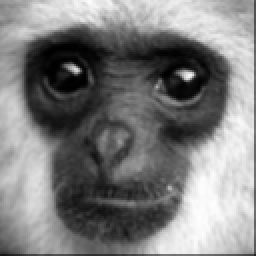
\includegraphics[width=0.2\linewidth]{result_1.jpg}
	\caption{Фрактальное сжатие}
	\label{fig:mpr}
\end{figure}

\begin{figure}[h]
	\centering
	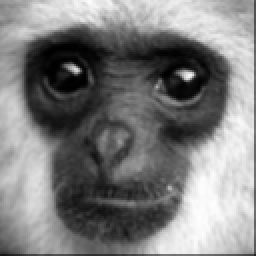
\includegraphics[width=0.2\linewidth]{result_ultra_mega_sposob_1.jpg}
	\caption{Способ сохранения}
	\label{fig:mpr}
\end{figure}

\subsubsection{6 в 3}
\begin{figure}[h]
	\centering
	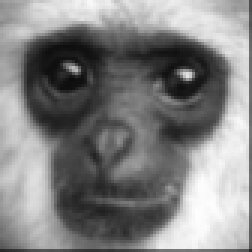
\includegraphics[width=0.2\linewidth]{result_11.jpg}
	\caption{Фрактальное сжатие}
	\label{fig:mpr}
\end{figure}

\begin{figure}[h]
	\centering
	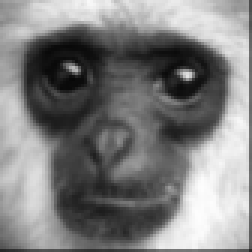
\includegraphics[width=0.2\linewidth]{result_ultra_mega_sposob_11.jpg}
	\caption{Способ сохранения}
	\label{fig:mpr}
\end{figure}

\subsubsection{8 в 4}
\begin{figure}[h]
	\centering
	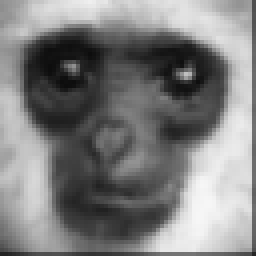
\includegraphics[width=0.2\linewidth]{result_12.jpg}
	\caption{Фрактальное сжатие}
	\label{fig:mpr}
\end{figure}

\begin{figure}[h]
	\centering
	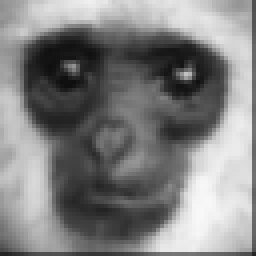
\includegraphics[width=0.2\linewidth]{result_ultra_mega_sposob_12.jpg}
	\caption{Способ сохранения}
	\label{fig:mpr}
\end{figure}

\subsubsection{10 в 5}
\begin{figure}[h]
	\centering
	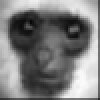
\includegraphics[width=0.2\linewidth]{result_13.jpg}
	\caption{Фрактальное сжатие}
	\label{fig:mpr}
\end{figure}

\begin{figure}[h]
	\centering
	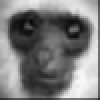
\includegraphics[width=0.2\linewidth]{result_ultra_mega_sposob_13.jpg}
	\caption{Способ сохранения}
	\label{fig:mpr}
\end{figure}

\subsection{Большое изображение}
\subsubsection{4 в 2}
Из-за долгого времени работы алгоритма, на большом изображения такое маленькое разбиение не тестировалось.

\subsubsection{6 в 3}
\begin{figure}[h]
	\centering
	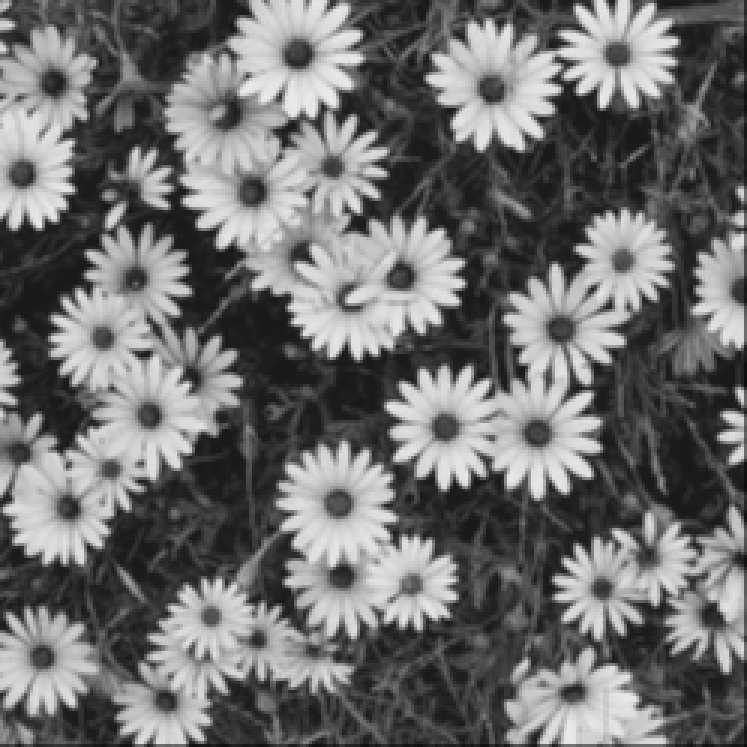
\includegraphics[width=0.2\linewidth]{result_2.jpg}
	\caption{Фрактальное сжатие}
	\label{fig:mpr}
\end{figure}

\begin{figure}[h]
	\centering
	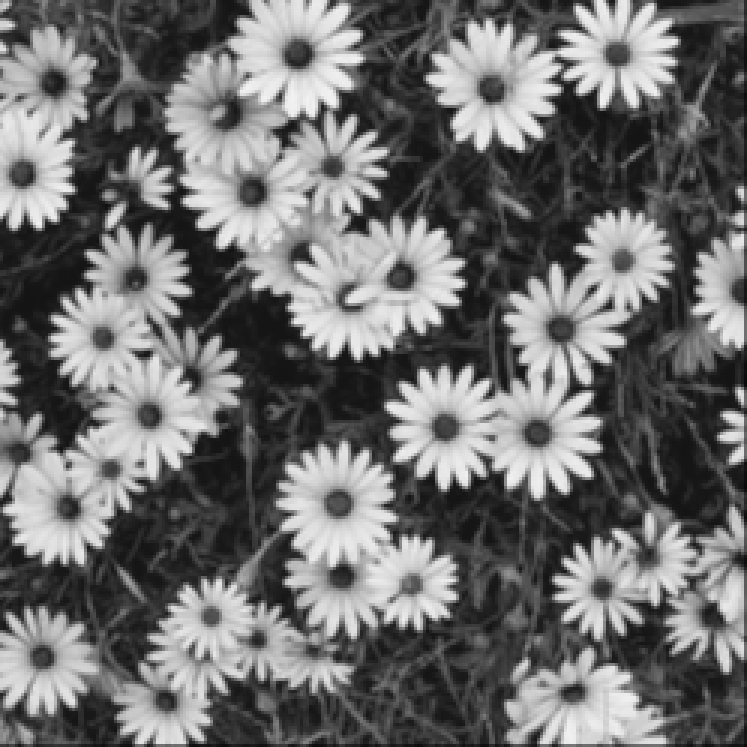
\includegraphics[width=0.2\linewidth]{result_ultra_mega_sposob_2.jpg}
	\caption{Способ сохранения}
	\label{fig:mpr}
\end{figure}

\subsubsection{8 в 4}
\begin{figure}[h]
	\centering
	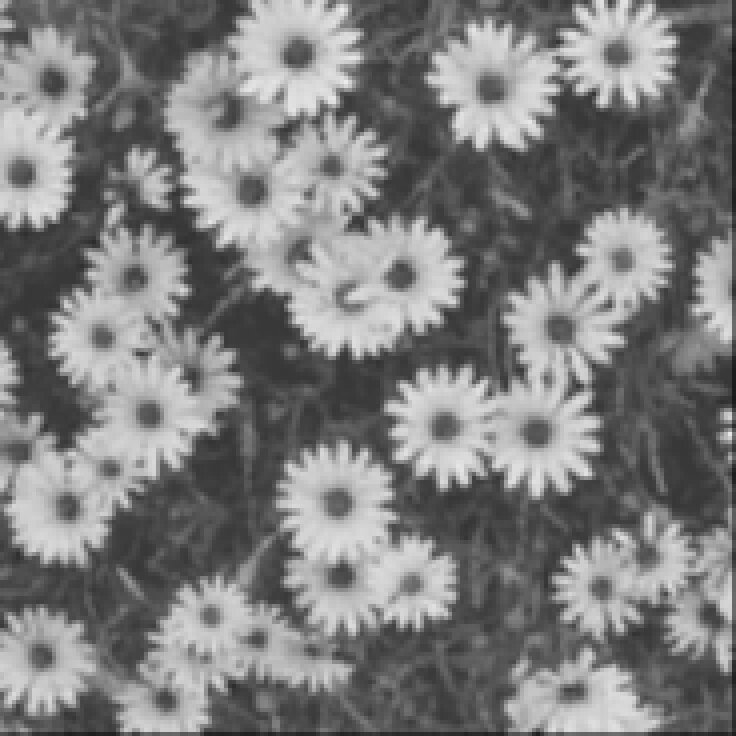
\includegraphics[width=0.2\linewidth]{result_22.jpg}
	\caption{Фрактальное сжатие}
	\label{fig:mpr}
\end{figure}

\begin{figure}[h]
	\centering
	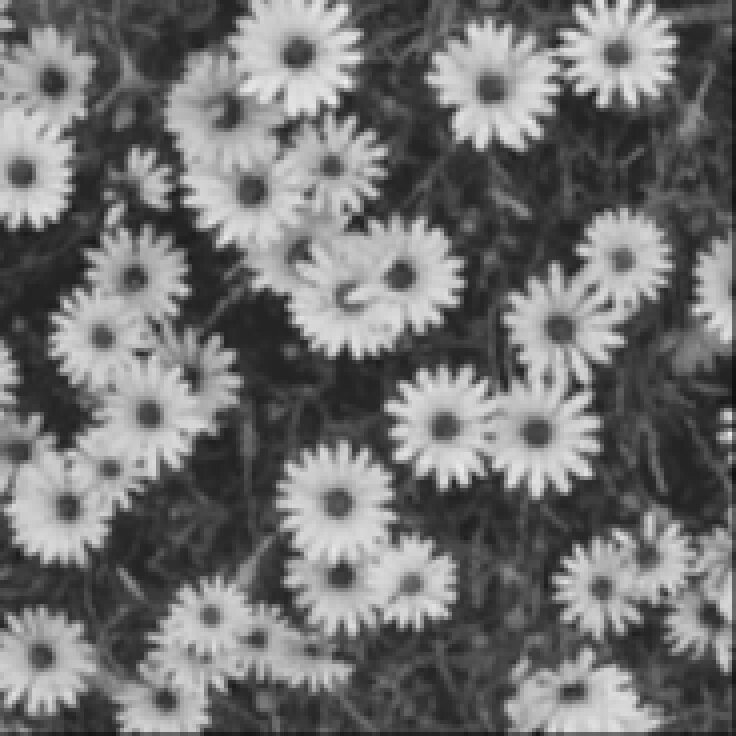
\includegraphics[width=0.2\linewidth]{result_ultra_mega_sposob_22.jpg}
	\caption{Способ сохранения}
	\label{fig:mpr}
\end{figure}

\subsubsection{10 в 5}
\begin{figure}[h]
	\centering
	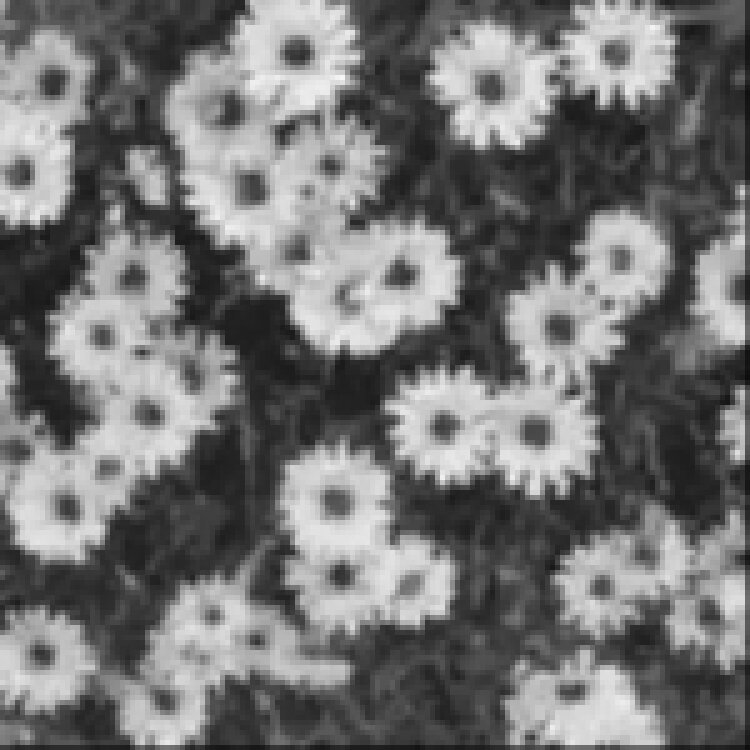
\includegraphics[width=0.2\linewidth]{result_23.jpg}
	\caption{Фрактальное сжатие}
	\label{fig:mpr}
\end{figure}

\begin{figure}[h]
	\centering
	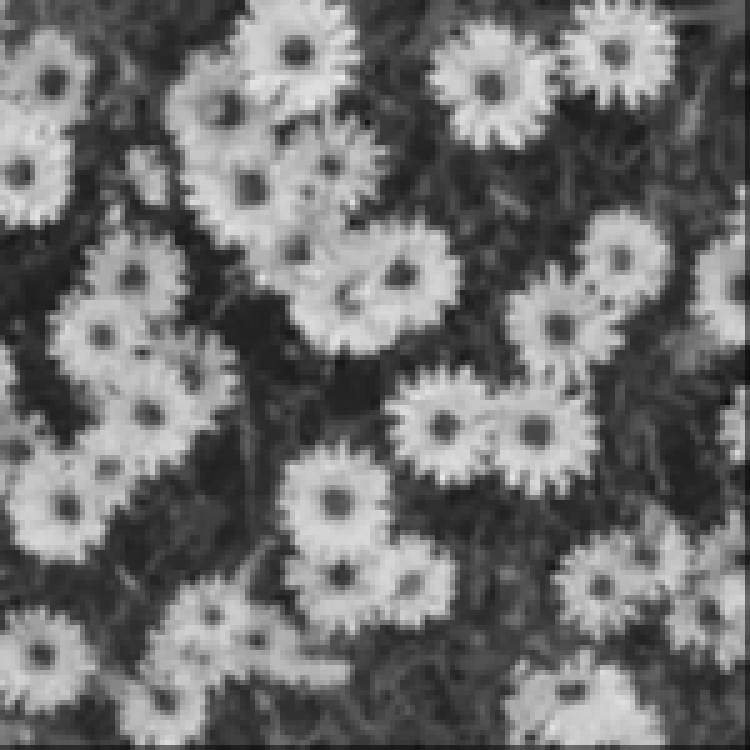
\includegraphics[width=0.2\linewidth]{result_ultra_mega_sposob_23.jpg}
	\caption{Способ сохранения}
	\label{fig:mpr}
\end{figure}

\subsection{Опрос}

Для выявления лучших коэффициентов сжатия было опрошено 8 человек и получены следующие результаты:

Для маленького изображения:

\begin{center}
	\begin{tabular}{||c c c c c c c c c c c c c||} 
		\hline
		Коэффициент сжатия & Респондент 1 & Респондент 2 & Респондент 3 & Респондент 4 & Респондент 5 & Респондент 6 & Респондент 7 & Респондент 8 & Средняя оценка & Время работы & Размер в сжатом виде(Кб) & Исходный размер(Кб) \\ [0.5ex] 
		\hline\hline
		4 в 2 фрак & 6,5 & 6 & 6 & 6 & 9 & 9 & 9 & 5 & 7,0625 & 0:14:09.624059 & 193 & 193 \\ 
		\hline
		4 в 2 сохр & 5	& 3 & 3 & 5 & 7 & 9 & 9 & 5,5 &	5,8125 & 0:14:09.624059 & 129 &	193 \\
		\hline
		6 в 3 фрак & 5 & 5 & 5 & 5 & 6 & 7 & 6 & 4 &	5,375 & 0:00:28.290035 & 37 &	193 \\
		\hline
		6 в 3 сохр & 3 & 3 & 2 & 4 & 5 & 7 & 6 & 4,5 &	4,3125 & 0:00:28.290035 & 56 &	193 \\
		\hline
		8 в 4 фрак & 3,5 &	6 &	1 &	3 &	5 &	8 &	7 &	1 &	4,3125 & 0:00:03.945229 & 13 &	193 \\ 
		\hline
		8 в 4 сохр & 2 & 2 & 1 & 3 & 3 & 8 & 7 & 1,5 &	3,4375 & 0:00:03.945229 & 33 &	193 \\ 
		\hline
		10 в 5 фрак & 2,5 & 4 &	1 &	2 &	4 &	6 &	5  & 0,5 &	3,125 &	0:00:01.207121 & 5 & 193 \\ 
		\hline
		10 в 5 сохр & 1 & 3 & 1 & 2 & 3 & 6 & 5 & 1 & 2,75 & 0:00:01.207121 & 20 & 193 \\ [1ex] 
		\hline
	\end{tabular}
\end{center}

Для большого изображения:

\begin{center}
	\begin{tabular}{||c c c c c c c c c c c c c||} 
		\hline
		Коэффициент сжатия & Респондент 1 & Респондент 2 & Респондент 3 & Респондент 4 & Респондент 5 & Респондент 6 & Респондент 7 & Респондент 8 & Средняя оценка & Время работы & Размер в сжатом виде(Кб) & Исходный размер(Кб) \\ [0.5ex] 
		\hline\hline
		4 в 2 фрак & - & - & - & - & - & - & - & - & - & - & - & - \\ 
		\hline
		4 в 2 сохр & - & - & - & - & - & - & - & - & - & - & - & - \\
		\hline
		6 в 3 фрак & 5 & 5 & 7 & 5 & 6 & 7 & 6 & 4 &	5,625 & 0:34:20.081393 & 324 &	209 \\
		\hline
		6 в 3 сохр & 3 & 3 & 2 & 4 & 5 & 7 & 6 & 4,5 &	4,3125 & 0:34:20.081393 & 485 &	209 \\
		\hline
		8 в 4 фрак & 3,5 &	6 &	1 &	3 &	5 &	8 &	7 &	1 &	4,3125 & 0:03:39.547086 & 100 &	209 \\ 
		\hline
		8 в 4 сохр & 2 & 2 & 1 & 3 & 3 & 8 & 7 & 1,5 &	3,4375 & 0:03:39.547086 & 265 &	209 \\ 
		\hline
		10 в 5 фрак & 1,5 & 3 &	1 &	1 &	3 &	4 &	3  & 0,5 &	3,125 &	0:00:38.118574 & 43 & 209 \\ 
		\hline
		10 в 5 сохр & 1 & 2 & 1 & 1 & 2 & 4 & 3 & 1 & 1,875 & 0:00:38.118574 & 176 & 209 \\ [1ex] 
		\hline
	\end{tabular}
\end{center}

Из результатов опроса видно, что для малых изображений лучше всего использовать сжатие 6 в 3, т.к. оно не сильно затратно по времени и имеет хорошую четкость. Для больших изображений лучше использовать сжатие 8 в 4, хотя при таком сжатия существенно падает качество изображения, но время затраченное на это не столь велико.

  
\end{document}